%% LyX 2.3.0 created this file.  For more info, see http://www.lyx.org/.
%% Do not edit unless you really know what you are doing.
\documentclass[12pt,english]{article}
\usepackage{mathptmx}
\renewcommand{\familydefault}{\rmdefault}
\usepackage[T1]{fontenc}
\usepackage[latin9]{inputenc}
\usepackage{geometry}
\geometry{verbose,tmargin=2cm,bmargin=2cm,lmargin=2cm,rmargin=2cm}
\usepackage{float}
\usepackage{graphicx}

\makeatletter
%%%%%%%%%%%%%%%%%%%%%%%%%%%%%% User specified LaTeX commands.
\usepackage{lineno} 
\linenumbers


\usepackage{xr}
\externaldocument{coexistence_species-rich}

\makeatother

\usepackage{babel}
\begin{document}
\emph{Supplementary Material} for \textbf{How self-regulation, the storage effect and their interaction contribute to coexistence in stochastic and seasonal environments}- Picoche, C. \& Barraquand, F.

\appendix

\section{Supplementary Figures}

\renewcommand\thefigure{\thesection.\arabic{figure}} 

\begin{figure}[H]
\begin{centering}
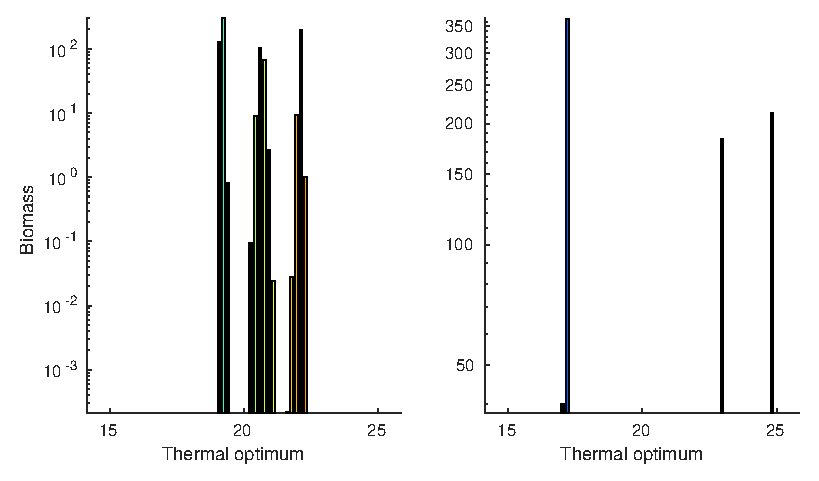
\includegraphics[width=0.95\textwidth]{graphe/FigS1}
\par\end{centering}
\caption{Temporal mean of biomass a function of the thermal optimum defining
each species. The temporal means are computed over the last 200 years
of a simulation spanning 5000 years. We considered both a white noise
(left) or a seasonal forcing signal (right). The coexistence mechanism
implemented is the storage effect, and no stabilizing niche differences
were considered (same inter- and intra-specific competition). This
simulation is the one described in Fig. 1
in main text\label{fig:Appendix_mean_biomass_iter2}. 99 other simulations
have been performed to produce the main text results in Figs. 2-4. }
\end{figure}

\begin{figure}[H]
\begin{centering}
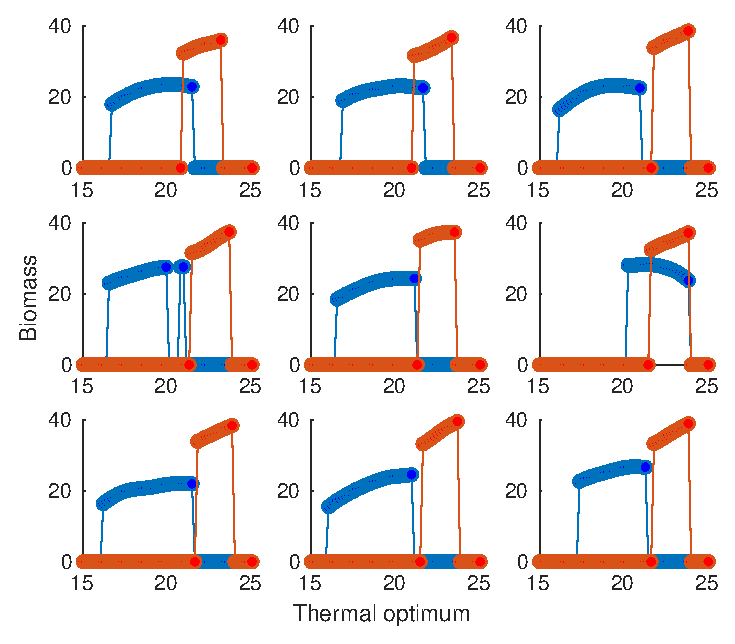
\includegraphics[width=0.95\textwidth]{graphe/example_iteration}
\par\end{centering}
\caption{Temporal mean biomass distribution, computed over the last 200 years,
for 9 representative simulations, as a function of the thermal optimum
of the species. These simulations are done without storage effect
but with strong self-regulation. Temperature is either a seasonal
signal (in red) or a random noise (in blue). The distribution induced
by a white noise forcing overlaps the one obtained with a seasonal
forcing signal in only 2 simulations out of 100, hence the two signals
lead in general to very different biomass distributions on the environmental
trait axis. \label{fig:Not_representative_behaviour} }
\end{figure}

\end{document}
